\documentclass[12pt,a4paper,italian]{article}


\usepackage[italian]{babel}
\usepackage[latin1]{inputenc}
\usepackage{amsmath}
\usepackage{amsfonts}
\usepackage{amssymb}
\usepackage{color}
\usepackage{xcolor}
\usepackage{hyperref}
\usepackage[all]{hypcap}
\usepackage{ifthen}
\usepackage{wrapfig}
%\author{Piero Bizzotto}
\usepackage[top=2cm,bottom=5cm,left=80pt,right=80pt]{geometry}
\usepackage{graphicx}
\DeclareGraphicsExtensions{.jpg,.png}

\newcommand{\ajax}{AJAXDRAW}
\newcommand{\sito}{\href{http://ajaxdraw.sourceforge.net}{http://ajaxdraw.sourceforge.net}}

\setlength{\parindent}{0pt} %settato indentazione di default 
\setlength{\headheight}{3cm} %settato grandezza header...in altre parole, quanto distanzio il doc dall'intestazione

\usepackage{fancyhdr} %pacchetto per le intestazioni
\pagestyle{fancy} %uso del pacchetto


\fancyhead{} %annulla head di default
\fancyfoot{} %annulla foot di default


\usepackage{lastpage} %setto pg di pgtot a rfoot
     \rfoot{pagina \thepage\ di \pageref{LastPage}}


\lfoot{Versione: \insertversion} %setto versione doc a lfoot
\renewcommand{\footrulewidth}{0.5pt} %ridefinisco il valore della riga di intestazione
\renewcommand{\headrulewidth}{0.5pt} %ridefinisco il valore della riga di pie' di pagina

\newcommand{\insertversion}{0.0} %definisco il nuovo comando per inserire la versione


\lhead{  \begin{Huge} \ajax \end{Huge} \\  %intestazione di sinistra
					%\begin{Large}	Software per il Disegno Grafico\\ in Tecnologie Web \end{Large}  
					\begin{normalsize}\sito \end{normalsize}
			%\\ versione documento: \insertversion\ del \today} %setto l'intestazione sx
		}
\rhead{ %includo logo nell'intestazione dx
	 	
\includegraphics[scale=0.5]{../logo/logo.png}  
}


%CREAZIONE ELENCHI NUMERATI PERSONALIZZATI
\newcounter{Lcount}
\newcounter{Rcount}
\setcounter{Lcount}{0}
\setcounter{Rcount}{0}

\newenvironment{elenconumerato}[2][ ]
{
  \begin{list}{#1\arabic{Lcount}.}
    {
	\setcounter{Rcount}{\value{Lcount}}
	\setcounter{Lcount}{0} 
	\usecounter{Lcount} 
\addtolength{\leftmargin}{#2pt}
	}
}
{
  \end{list}
 \setcounter{Lcount}{\value{Rcount}}
}

%CREAZIONE ELENCHI PUNTATI
\newenvironment{elencopuntato}[1][]
{
\begin{list}{\textbullet} %\itemindent=#1pt
	{
	\addtolength{\leftmargin}{#1pt}
	}
} 
{
\end{list}
}


\newenvironment{elencodescrittivo}[1][]{\begin{description} \setlength{\itemindent}{#1pt} \addtolength{\leftmargin}{#1pt}} {\end{description}}

\newcommand{\TITOLODOC}{Titolo}

%footer centrale
\cfoot{ \TITOLODOC \\  E-mail:    \href{ mailto:webshape.contact@gmail.com}{ webshape.contact@gmail.com}  }

%INSERIMENTO IMMAGINI
\newcommand{\imagerealsize}[1]{\vspace{20pt} \includegraphics{#1} }
\newcommand{\imageadapted}[1]{\vspace{20pt} \includegraphics[width=1\textwidth]{#1} }

\newcommand{\glosspath}{.\glossario}
\newcommand{\gloss}[1]{\hyperref{\glosspath~\glossario.pdf}{}{#1}{#1}}

\hypersetup{
    %bookmarks=true,         % show bookmarks bar?
    %unicode=false,          % non-Latin characters in Acrobat’s bookmarks
	%pdftoolbar=true,        % show Acrobat’s toolbar?
	%pdfmenubar=true,        % show Acrobat’s menu?
    %pdffitwindow=true,      % page fit to window when opened
    %pdftitle={My title},    % title
    %pdfauthor={Author},     % author
    %pdfsubject={Subject},   % subject of the document
    %pdfnewwindow=true,      % links in new window
    %pdfkeywords={keywords}, % list of keywords
    colorlinks=true,         % false: boxed links; true: colored links
    linkcolor=black,           % color of internal links
    %citecolor=green,        % color of links to bibliography
    %filecolor=magenta,      % color of file links
    urlcolor=teal    % color of external links
%	linktocpage=false;
}


%COLORAZIONE TESTO
\newcommand{\blue}[1]{{\color {blue} #1}} 
\newcommand{\red}[1]{{\color {red} #1}}
\newcommand{\green}[1]{{\color {green} #1}}
\newcommand{\sezione}[1]{\leftskip=0pt \section{#1} \leftskip=18pt}
\newcommand{\subsezione}[1]{\leftskip=18pt \subsection{#1} \leftskip=36pt}
\newcommand{\subsubsezione}[1]{\leftskip=36pt \subsubsection{#1} \leftskip=54pt}
\newcommand{\subsubsecindent}{54}
\newcommand{\subsecindent}{36}
\newcommand{\secindent}{18}
\newcommand{\normindent}{8}
\newcommand{\code}[1]{{\bfseries \texttt{#1}}}
\newcommand{\paragrafo}[1]{\leftskip=36pt \paragraph{#1} \leftskip=54pt}
\newcommand{\subparagrafo}[1]{\leftskip=54pt \subparagraph{#1} \leftskip=72pt} %BASE!!!
\usepackage{multirow}
\title{\TITOLODOC}
\author{Marco Cunico}

\begin{document}

\renewcommand{\insertversion}{0.0} %INSERIRE LA VERSIONE QUI DENTRO STILE x.x.xx
\renewcommand{\TITOLODOC}{Manuale Utente} %INSERIRE IL TITOLO DEL DOCUMENTO DA FAR COMPARIRE A PIE PAGINA
\renewcommand{\glosspath}{.\glossario} %INSERIRE PERCORSO RELATIVO

%%%%%%%%%%%%%%%%%%%%%%PARTE DA NON MODIFICARE%%%%%%%%%%%%%%%%%
\begin{titlepage}
\begin{center}
	\begin{Large}	\today \end{Large}
\end{center}

\vspace{20pt}

\begin{center}
	\begin{Huge}
				\textbf{\ajax}
	\end{Huge}
\end{center}			

\begin{center}
	\begin{large}
				\textbf{Software per il Disegno Grafico\\ in Tecnologie Web}
	\end{large}
\end{center}			

\vspace{20pt}

\begin{center}

\includegraphics[width=150pt]{../logo/logo}
\end{center}

\vspace{170pt}
\begin{center} %INSERIRE ALL'INTERNO IL TITOLO DOCUMENTO CHE COMPARIRA NELLA PAGINA INIZIALE				
	\begin{Huge}
				\textbf{\TITOLODOC}
	\end{Huge}
			\\
\end{center}
\vspace{190pt}
\begin{center}
Versione: \insertversion
\end{center}
\end{titlepage}

\newpage
%%%%%%%%%%%%%%%%%%%%%%FINE PARTE DA NON MODIFICARE%%%%%%%%%%%%%%%%%

\begin{center} %INSERIRE ALL'INTERNO IL TITOLO DOCUMENTO CHE COMPARIRA NELLA PAGINA INIZIALE
	\begin{Huge}	
				\textbf{\TITOLODOC}
			\\
	\end{Huge}
\end{center}

%\setlength{\parindent}{18pt} %settato indentazione di default 
\section*{\LARGE Sommario:}
Il presente documento si propone di fornire la documentazione di supporto necessaria per l'utilizzo del prodotto.

 %SEZIONE SOMMARIO
\indent \indent

\section*{\LARGE Stato del documento:}
\indent \indent
	Formale Esterno

\section*{\LARGE Redazione:}
	\begin{table}[!h]
		\begin{center}
			\begin{tabular}
				{|c|c|}
				\hline
				%%%%%%%%%%%%%%INTESTAZIONE COLONNE%%%%%%%%%%%%%%%%%%%%%%%%%%%%%%%%
				\multicolumn{2}{|c|}{ \textbf{Redazione} } \\
				\hline
				\textbf{Fase} & \textbf{Redattori} \\
				%%%%%%%%%%%%%%FINE INTESTAZIONE COLONNE%%%%%%%%%%%%%%%%%%%%%%%%%%%%%%%%%%%%%%
				\hline
				%%%%%%%%%%% PARTE DA MODIFICARE %%%%%%%%%%%%%%%%%%%%%%%%%%%%%%%%%%%%%%%%%%		
				\multirow{2}{*}{PPP-RQ} & \\
										& \\
				\hline
				%%%%%%%%%%% FINE PARTE DA MODIFICARE %%%%%%%%%%%%%%%%%%%%%%%%%%%
			\end{tabular}
			\caption{Lista Redattori} %INSERIRE DIDASCALIA - SE NECESSARIA - 
			\label{tabredazione}
		\end{center}
	\end{table}
	
	
\section*{\LARGE Approvazione:}
\begin{table}[!h]
	\begin{center}
		\begin{tabular}
			{|c|c|}
			\hline
			%%%%%INTESTAZIONE COLONNE%%%%%%%%%%%%%%%%%%%%%%%%%%%%%%%
			\multicolumn{2}{|c|}{ \textbf{Approvazione} } \\
			\hline
			\textbf{Fase} & \textbf{Approvatori} \\
			%%%%%%%%%%%%%%FINE INTESTAZIONE COLONNE%%%%%%%%%%%%%%%%%%%%%%%%%%%%%%
			\hline
			%%%%%%%%%%% PARTE DA MODIFICARE %%%%%%%%%%%%%%%%%%%%%%%%%%%%%%%%%%%%%%		
			\multirow{1}{*}{RPP-RQ} & \\
									
			\hline
			%%%%%%%%%%% FINE PARTE DA MODIFICARE %%%%%%%%%%%%%%%%%%%%%%%%%%%%%%%%%%%
		\end{tabular}
		\caption{Lista Approvatori} %INSERIRE DIDASCALIA - SE NECESSARIA - 
		\label{tabapprovazione}
	\end{center}
\end{table}

\textbf{}
\newpage
\section*{\LARGE Lista di Distribuzione:}

	\begin{elenconumerato}{\normindent}
		\item WebShape 
		\item I committenti Conte Renato e Vardanega Tullio in rappresentanza \\  dell'azienda proponente Zucchetti SPA
	\end{elenconumerato}




\section*{\Large Registro delle Modifiche:}


\begin{center}
	\begin{table}[h]
		  \begin{tabular*}
			{1\textwidth}%
				{@{\extracolsep{\fill}}|p{0.1\textwidth}|p{0.54\textwidth}|p{0.26\textwidth}|}
			 \hline
%%%%%%%%%%%%%%INTESTAZIONE COLONNE%%%%%%%%%%%%%%%%%%%%%%%%%%%%%%%%%%%%%%%%%%
			\textbf{Versione}  & \textbf{Descrizione} & \textbf{Autore} \\
%%%%%%%%%%%%%%FINE INTESTAZIONE COLONNE%%%%%%%%%%%%%%%%%%%%%%%%%%%%%%%%%%%%%%%
		 \hline
%%%%%%%%%%% PARTE DA MODIFICARE %%%%%%%%%%%%%%%%%%%%%%%%%%%%%%%%%%%%%%%%%%%
    	  \hline
    	  0.0 & 27/02/2008 Prima stesura & \\

		\hline %%FINE RIGA
%%%%%%%%%%% FINE PARTE DA MODIFICARE %%%%%%%%%%%%%%%%%%%%%%%%%%%%%%%%%%%%%
		\end{tabular*}
	\caption{Registro delle modifiche} %INSERIRE DIDASCALIA - SE NECESSARIA - 
	\label{tab:modifiche}
	\end{table}
\end{center}


\newpage
\thispagestyle{fancy}
\tableofcontents
\thispagestyle{fancy}
\newpage

\sezione{Introduzione}

\subsezione{Definizione dell'utente del prodotto}
Il prodotto \`e pensato per tutti gli utenti che hanno conoscenze minime in ambiente di grafica vettoriale e che possiedono una connessione ad internet. Il sistema potr\`a essere modificato da chiunque voglia estendere l'applicazione, secondo le norme che regolano la licenza d'utilizzo.\\

\subsezione{Come leggere il manuale}
Il presente Manuale Utente \`e suddiviso in varie sezioni. Nella sezione ''Introduzione'' il lettore pu\`o trovare riferimenti a documenti utili per l'uso del prodotto e informazioni riguardo eventuali segnalazioni di problemi riscontrati nel suo utilizzo.
Nella sezione ''Descrizione generale'' viene descritto il prodotto illustrandone lo scopo, le modalit\`a di utilizzo, le caratteristiche salienti, i requisiti tecnici. Nella sezione ''Istruzioni d'uso'' sono presenti le operazioni da effettuare per utilizzare il software, a partire dall'installazione fino al termine di una sessione di utilizzo.\\ %integrate anche mediante vari screenshot


\subsezione{Documenti Utili}
\begin{elencopuntato}[\normindent]
	\item[-] \textit{Glossario.pdf}
\end{elencopuntato}

\subsezione{Come riportare problemi e malfunzionamenti}
Nel caso durante l'utilizzo del prodotto sorgano problemi o malfunzionamenti non descritti nel seguente documento, l'utente \`e invitato a contattare la WebShape all'indirizzo \href{mailto:webshape.contact@gmail.com}{webshape.contact@gmail.com} riportando i seguenti dati:\\
\begin{elencopuntato}[\normindent]
	\item[-] Versione del prodotto;
	\item[-] Sistema operativo in uso;
	\item[-] \underline{Browser} in uso;
	\item[-] Configurazione hardware in uso;
	\item[-] Fase di utilizzo in cui si \`e manifestato l'errore;
	\item[-] Descrizione dell'errore.
\end{elencopuntato}

\sezione{Descrizione Generale}

\subsezione{Caratteristiche del Prodotto}
Il prodotto \`e stato sviluppato come un'applicazione web. \`E possibile utilizzarlo, una volta installato sul \underline{server}, semplicemente accedendovi tramite un browser. Una volta effettuato l'accesso alla pagina \`e possibile accedere a tutte le
funzionalit\`a. Il sistema permette un salvataggio dei disegni che potranno essere ricaricati e aggiornati.

\subsezione{Requisiti tecnici per il funzionamento del programma}
\subsubsezione{Lato client}
\begin{elencopuntato}[\normindent]
    \item[-] Requisiti software: Firefox 3.1b2 o successivo, Firefox 3.0.6 tutto tranne il disegno di testo, Opera 9.6 tutto tranne il disegno di testo, Chrome (versione attuale), Safari (versione attuale), IE8: tutto tranne il testo e la selezione che risulta non essere ottimale.\\
    Risoluzione minima consigliata: 1024x768.\\
N.B. Dove non \`e supportato il testo, c'\`e un supporto minimo: un solo font, colore di riempimento ignorato, set di caratteri minimo. 
    \item[-] Requisiti hardware:  Processore Intel 2GHz o compatibili; 512MB memoria RAM 
\end{elencopuntato}
\subsubsezione{Lato server}
\begin{elencopuntato}[\normindent]
    \item[-] Requisiti software:  \underline{JVM} 1.5 o superiore, Apache \underline{Tomcat} 6.0 o superiore.
    \item[-] Requisiti hardware:  Processore Intel 1GHz; 1GB memoria RAM
\end{elencopuntato}

\sezione{Istruzioni per l'uso}

\subsezione{Installazione del programma}
\subsubsezione{Lato client}
Il programma non necessita di installazione. 

\subsubsezione{Lato server}

Per permettere il funzionamento del sistema, \`e necessario installare un Web Server: Apache Tomcat. Oltre ad essere un Web Server, Tomcat \`e anche un
Application Server, cio\`e una piattaforma per l'esecuzione di applicazioni Web sviluppate nel linguaggio Java.\\
\\
Prima di tutto \`e necessario disporre di una Java Virtual Machine. Per il download visitare il link al sito ufficiale della Sun Microsystem:\\
\href{http://java.com/download/index.jsp}{http://java.com/download/index.jsp}\\
\\
Per effettuare il download di Apache Tomcat 6.0 seguire il link del sito ufficiale: \href{http://tomcat.apache.org/download-60.cgi}{http://tomcat.apache.org/download-60.cgi}\\

Nella sezione \textit{Binary Distribution} della pagina web, \`e possibile effettuare il download sia per sistemi Windows che per sistemi Linux.\\
\\
\indent{\textbf{Installazione su sistemi Windows:}}\\

Terminato il download, aprire il file scaricato per iniziare l'installazione.\\
\\
La schermata \`e la seguente:

\begin{figure}[!ht]
\centering
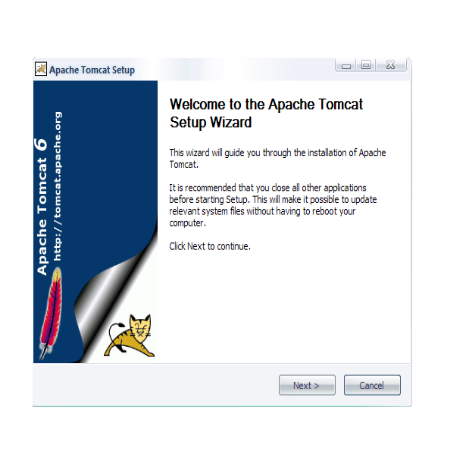
\includegraphics[scale=0.7]{images/InstallTomcat1.png}
\caption{Setup Wizard Apache Tomcat}
\end{figure} 

Premere \textit{Next} per proseguire e accettare la licenza.
Giunti alla schermata per la scelta della cartella di installazione, mantenere quella indicata di default.

\begin{figure}[!ht]
\centering
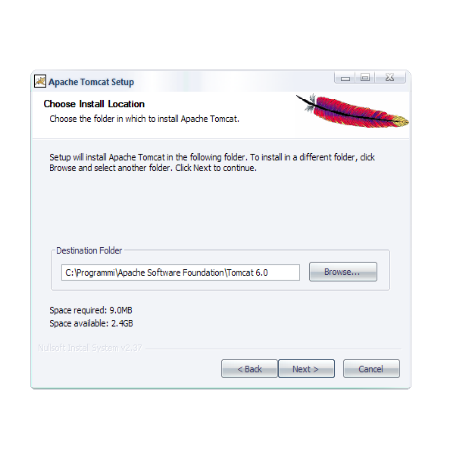
\includegraphics[scale=0.7]{images/InstallTomcat2.png}
\caption{Choose Install Location}
\end{figure} 
\newpage

Premere \textit{Next}, e si presenter\`a la finestra di configurazione di Tomcat:
Alla voce \textit{http/1.1 Connector Port} mantenere il valore di default (solitamente 8080), quindi impostare Username e Password, necessarie per accedere alla configurazione di Tomcat.\\
Quindi premere \textit{Next}.



\begin{figure}[!ht]
\centering
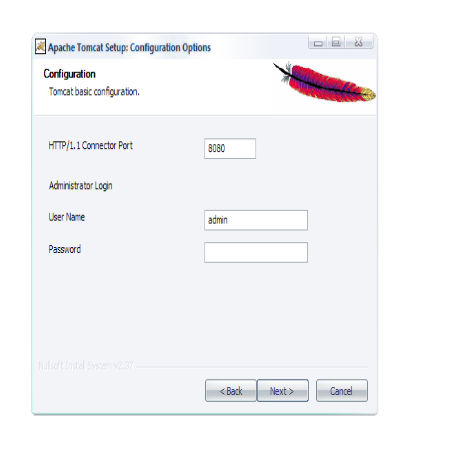
\includegraphics[scale=0.7]{images/InstallTomcat3.png}
\caption{Configuration}
\end{figure} 

Nella schermata successiva, \`e necessario indicare il percorso dell'installazione della Java Virtual Machine (J2SE). Se g\`a  installata, mantenere il percorso di default indicato. Per completare l'installazione, cliccare su \textit{Install}.

\begin{figure}[!ht]
\centering
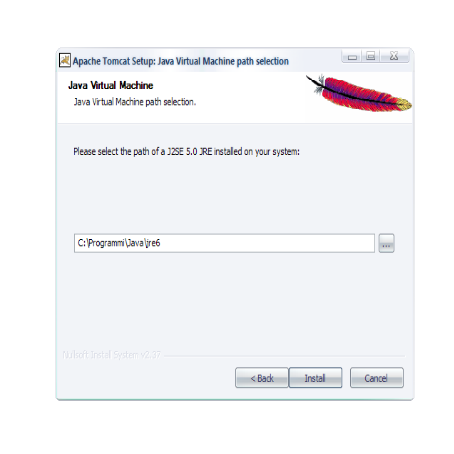
\includegraphics[scale=0.7]{images/InstallTomcat4.png}
\caption{Java Virtual Machine}
\end{figure} 

\indent{\textbf{Installazione su sistemi Linux:}}\\
Scaricato il file .tar.gz, estrarre il contenuto in una cartella. Non \`e necessaria un'installazione vera e propria e per la sua esecuzione si rimanda al paragrafo \textit{Avvio del programma} sezione \textit{Linux}.

\subsezione{Avvio del programma}
\subsubsezione{Lato client}
\`E sufficiente aprire la pagina web con un browser supportato. L'indirizzo dipende dall'host nel quale viene installato il web server.
\subsubsezione{Lato server}
Sono presenti due sezioni per effettuare l'avvio su sistemi Windows e su sistemi Linux.\\ \\ \\
\indent{\textbf{Avvio del programma su sistemi Windows:}}\\
Per l'avvio del web server, andare su \textit{Start-$ > $Programmi-$ > $Apache Tomcat 6.0} e avviare \textit{Monitor Tomcat}.
Nella barra delle applicazioni in esecuzione, apparir\`a l'icona che indica l'avvio di Tomcat.\\
A questo punto avviare un browser e digitare il seguente indirizzo:\\ 
\href{http://localhost:8080/manager/html}{http://localhost:8080/manager/html}\\
Dopo aver inserito Username e Password richiesti, si entrer\`a nell'area di gestione di Tomcat.\\
Andare nella sezione \textit{WAR file to deploy} della pagina.\\

%\\
%Scaricato il .tar.gz, estrarre il contenuto su una cartella. 
%Aprire una shell e posizionarsi sulla cartella estratta.
%A questo punto \`e necessario provare ad avviare il processo di Tomcat. Per farlo, eseguire i seguenti comandi:\\
\textit{cd bin}\\
\textit{./catalina.sh start}\\

%Se tutto è andato per il meglio. dovrebbe comparire una scritta tipo:\\
%\textit{Using CATALINA_BASE: /home/red/apache-tomcat-6.0.14}\\
%Using CATALINA_HOME: /home/red/apache-tomcat-6.0.14\\
%Using CATALINA_TMPDIR: /home/red/apache-tomcat-6.0.14/temp\\
%Using JRE_HOME: /usr/lib/jvm/java-6-sun-1.6.0.03\\
\\
%Avviare un browser e inserire l'indirizzo \textit{http://localhost:8080}\\
%Se compare la pagina principale di Tomcat, significa il Web Server funziona correttamente.
%A questo punto, \`e necessario procedere alla configurazione dell'utente amministratore per poter usare il Tomcat Manager.
%Per fare questo, da shell, spostarsi nella cartella principale di Tomcat ed eseguire i seguenti comandi:\\
%\textit{cd conf}\\
%\textit{sudo gedit tomcat-users.xml}\\
%Sostituire il file aperto, con il seguente codice:\\
%<?xml version='1.0' encoding='utf-8'?>\\
%<tomcat-users>\\
%  <role rolename="manager"/>\\
%  <role rolename="admin"/>\\
%  <user username="admin" password="admin" roles="manager"/>\\
%</tomcat-users> \\
%\\
%In questo modo \`e stato impostato uno User Name con valore \textit{admin} e una Password con valore \textit{admin]. Queste credenziali sono da usare per accedere al Tomcat Manager.\\
%A questo punto avviare un browser e digitare il seguente indirizzo\\ \textit{http://localhost:8080/manager/html}\\
%Dopo aver inserito User Name e Password richiesti, si entrer\`a nel manager di Tomcat.\\
%Andare nella sezione \textit{WAR file to deploy} della pagina.

\newpage

\begin{figure}[!ht]
\centering
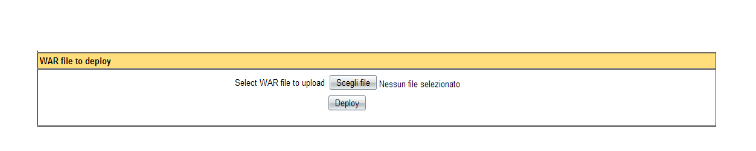
\includegraphics[scale=0.7]{images/DeployTomcat.png}
\caption{Deploy}
\end{figure} 


Selezionare il file \textit{.war} dell'applicazione e quindi cliccare su \textit{Deploy}.\\
A questo punto nella cartella \textit{webapps} della cartella di installazione di Tomcat sar\`a presente l'applicazione AJAXDRAW pronta per la sua esecuzione.\\ 
\\\\
\indent{\textbf{Avvio del programma su sistemi Linux:}}\\
Aprire una shell e posizionarsi sulla cartella di Apache Tomcat (precedentemente estratta).
A questo punto \`e necessario provare ad avviare il processo di Tomcat. Per farlo, eseguire i seguenti comandi:\\
\\
\textit{cd bin}\\
\textit{./catalina.sh start}\\

Se tutto \`e andato per il meglio, dovrebbero comparire i path di CATALINA e JRE.\\
%Using CATALINA_BASE: /home/red/apache-tomcat-6.0.14\\
%Using CATALINA\{_}HOME: /home/red/apache-tomcat-6.0.14\\
%Using CATALINA\{_}TMPDIR: /home/red/apache-tomcat-6.0.14/temp\\
%Using JRE\{_}HOME: /usr/lib/jvm/java-6-sun-1.6.0.03\\
\\
Avviare un browser e inserire l'indirizzo \href{http://localhost:8080}{http://localhost:8080}.\\
Se compare la pagina principale di Tomcat, significa che il Web Server funziona correttamente.
A questo punto, \`e necessario procedere alla configurazione dell'utente amministratore per poter utilizzare il Tomcat Manager.
Per fare questo, da shell, spostarsi nella cartella principale di Tomcat ed eseguire i seguenti comandi:\\
\\
\textit{cd conf}\\
\textit{sudo gedit tomcat-users.xml}\\
\\
Sostituire il contenuto del file aperto con il seguente codice:\\
\\
\textit{$ < $?xml version='1.0' encoding='utf-8'?$ > $}\\
\textit{$ < $tomcat-users$ > $}\\
\textit{  $ < $role rolename='manager'/$ > $}\\
\textit{  $ < $role rolename='admin'/$ > $}\\
\textit{  $ < $user username='admin' password='admin' roles='manager'/$ > $}\\
\textit{$ < $/tomcat-users$ > $} \\
\\
In questo modo \`e stato impostato uno Username con valore \textit{admin} e una Password con valore \textit{admin}. Queste credenziali possono essere utilizzate per accedere al Tomcat Manager.\\
A questo punto avviare un browser e digitare il seguente indirizzo\\ \href{http://localhost:8080/manager/html}{http://localhost:8080/manager/html}\\
Dopo aver inserito Username e Password richiesti, si acceder\` a al manager di Tomcat.\\
Raggiungere la sezione \textit{WAR file to deploy} della pagina.


\newpage
\begin{figure}[!ht]
\centering
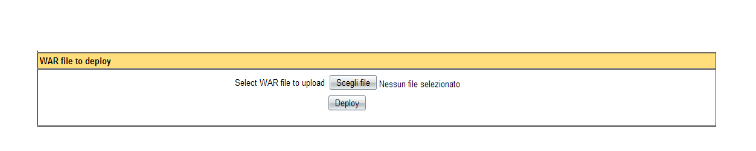
\includegraphics[scale=0.7]{images/DeployTomcat.png}
\caption{Deploy}
\end{figure} 

Selezionare il file .war dell'applicazione e quindi premere su Deploy.\\

\newpage

A questo punto nella cartella \textit{webapps} della cartella di installazione di Tomcat sar\`a presente l'applicazione AJAXDRAW pronta per la sua esecuzione. 



\subsezione{Descrizione funzionale - Lato client}
\subsubsezione{Il Menu}
Il programma dispone di un menu a tendina nella parte alta dell'interfaccia grafica.

\begin{figure}[!ht]
\centering
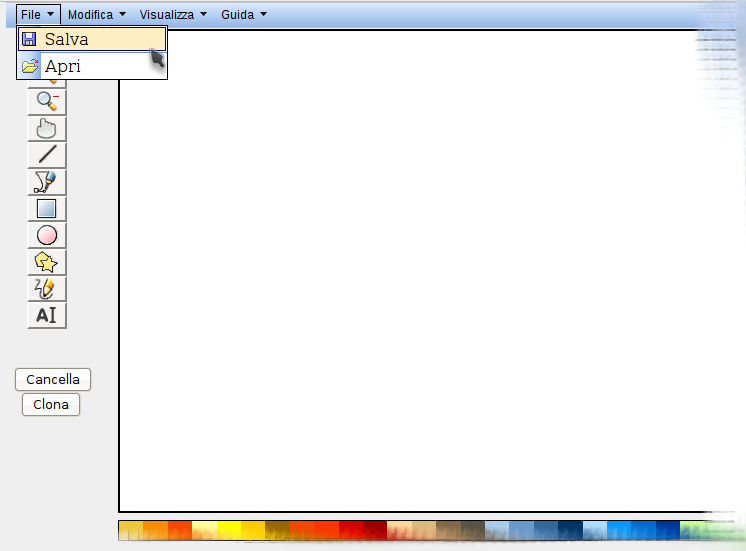
\includegraphics[scale=0.5]{images/menu.png}
\caption{menu a tendina}
\end{figure} 


Nella sezione \textit{File} \`e possibile salvare il lavoro svolto fino a quel momento sul proprio computer in formato \underline{svg}, oppure caricare un lavoro realizzato in precedenza.
Per aprire un file si deve selezionare \textit{File -$ > $Carica} e inserire il percorso del file nel dialog che si aprir\`a oppure selezionarlo cliccando sul pulsante \textit{Sfoglia}. 
Per salvare un file si deve selezionare \textit{File -$ > $Salva} e inserire un nome nel dialog che si aprir\`a in seguito e confermare la scelta. Comparir\`a un link che permette di scaricare il file.
La sezione \textit{Modifica} contiene il pulsante \textit{Svuota Canvas}, che permette di eliminare tutte le figure disegnate sul canvas e ricominciare dall'inizio.
La sezione \textit{Visualizza} permette di visualizzare i dialog delle propriet\`a nel caso fossero stati chiusi tramite il tasto di chiusura in alto a destra (la classica X). \textit{Colori} si riferisce alla finestra che modifica i colori di una figura mentre \textit{Propriet\`a} gestisce la posizione e la dimensione di una figura, e altre opzioni dipendenti dallo strumento in uso.
Infine la sezione \textit{Guida} contiene il link al manuale consultabile in linea, e permette di visualizzare informazioni sul prodotto e sull'azienda sviluppatrice.
\newpage

\subsubsezione{La Toolbar}
Le funzioni di disegno del programma sono accessibili attraverso i bottoni presenti nel lato sinistro dell'interfaccia grafica. Cliccando su un pulsante si attiva la funzione desiderata. Il puntatore del mouse cambia a seconda della funzione di disegno scelta, nei browser che lo supportano.


\begin{figure}[!ht]
\centering
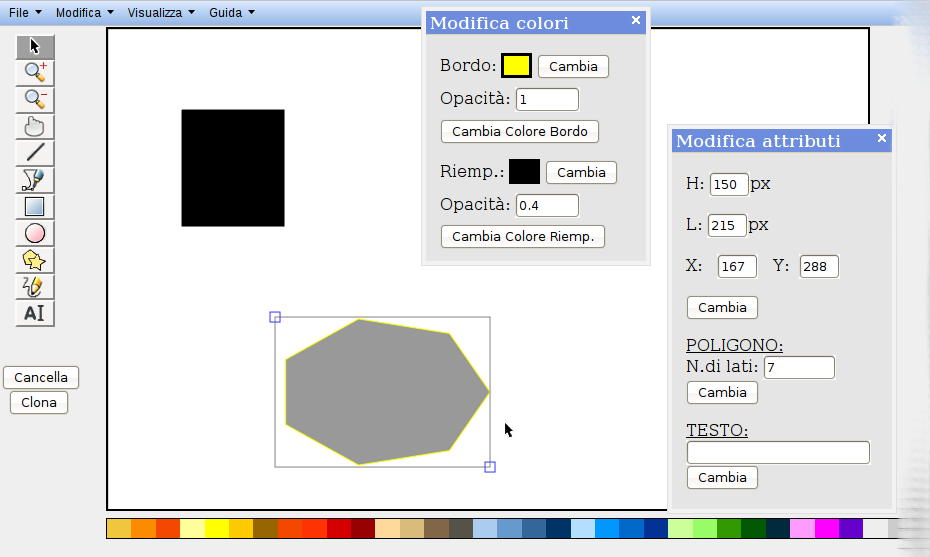
\includegraphics[scale=0.5]{images/selezione.png}
\caption{Selezione}
\end{figure} 

Qui \`e stata usata la funzione di \textit{selezione}. Una volta selezionata una figura, tutti i suoi parametri sono visualizzati nel dialog delle propriet\` a sulla destra. \`E possibile spostare i punti evidenziati cliccando su di essi e trascinare il mouse tenendo premuto il pulsante. Rilasciare il pulsante per fermare lo spostamento. Modificando questi punti \`e possibile regolare la dimensione delle figure, e nel caso specifico delle linee a mano libera e delle curve di Bezier si possono spostare i punti per cui passano le tangenti alle curve. Cliccando e mantenendo la pressione del pulsante sinistro del mouse all'interno di una figura, \`e possibile spostarla all'interno dell'area di disegno, azione effettuabile anche tramite le frecce direzionali della tastiera.

\begin{figure}[!ht]
\centering
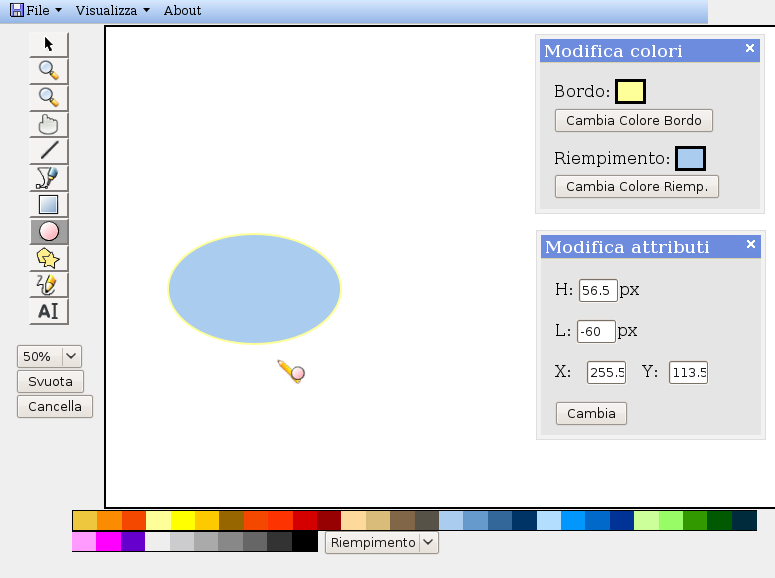
\includegraphics[scale=0.5]{images/ellisse.png}
\caption{Disegno di un Ellisse}
\end{figure} 

\vspace{100pt}
In questo caso \`e stata selezionata la funzione per il disegno di un'\textit{ellisse}. Cliccando e spostando il mouse sopra all'area disegnabile, si ha la possibilit\` a di creare una figura di dimensioni arbitrarie, che verr\` a effettivamente disegnata al rilascio del pulsante sinistro del mouse. Per il disegno di un \textit{rettangolo}, valgono le stesse considerazioni.
\newpage


\begin{figure}[!ht]
\centering
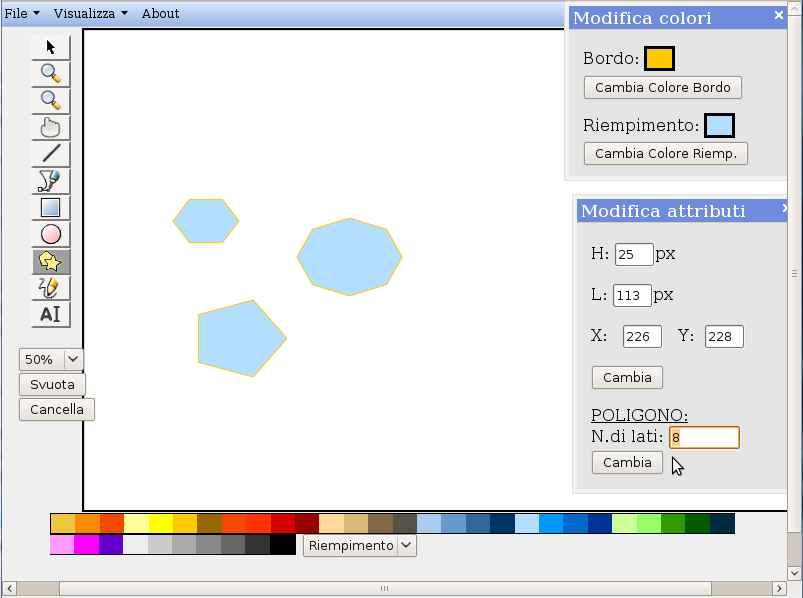
\includegraphics[scale=0.5]{images/poligono.png}
\caption{Disegno di un Poligono regolare}
\end{figure} 


\vspace{300pt}
Qui \`e stato disegnato un \textit{poligono regolare}. L'unica differenza rispetto ad ellissi e rettangoli consiste nella composizione della finestra di propriet\`a, alla quale si aggiunge una casella che permette di modificare il numero di lati del poligono da disegnare o disegnato, inserendo il valore desiderato a fianco dell'etichettta \textit{N. di lati} e confermando tale scelta cliccando sul pulsante \textit{Cambia}.


\newpage


\begin{figure}[!ht]
\centering
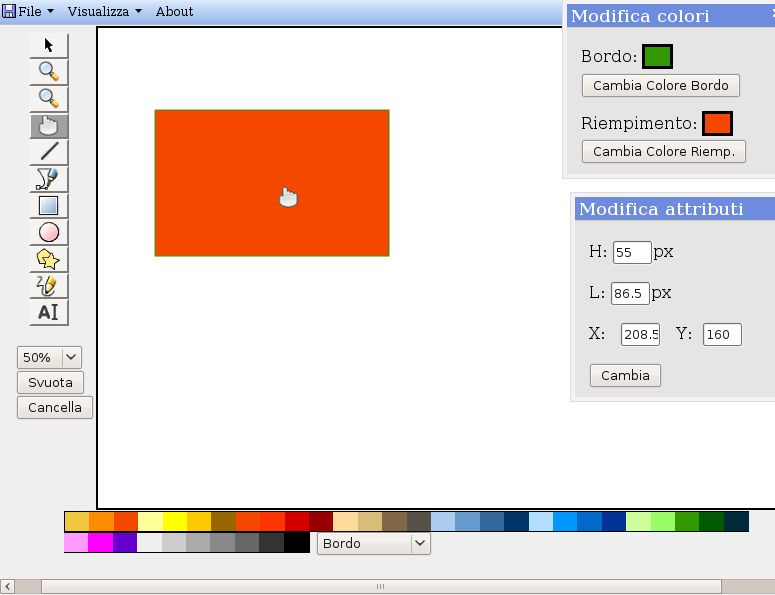
\includegraphics[scale=0.5]{images/mano.png}
\caption{Strumento Mano per spostare l'area visualizzata}
\end{figure} 


\vspace{100pt}
Qui \`e stata selezionata la funzione di \textit{spostamento} dell'area di disegno. Cliccando su un punto qualsiasi del \underline{canvas} \`e possibile cambiare l'area di disegno correntemente visualizzata spostando il mouse mantenendo premuto il tasto sinistro.
\newpage 


\begin{figure}[!ht]
\centering
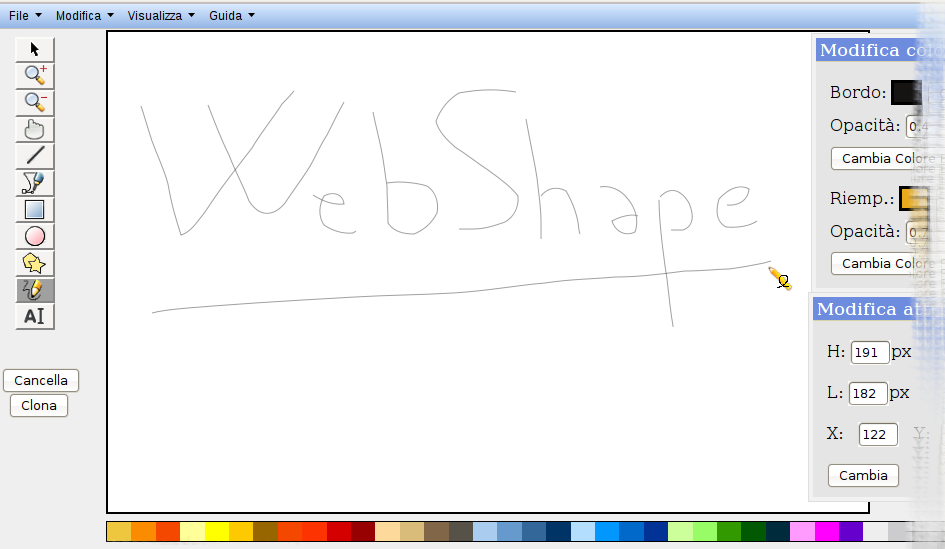
\includegraphics[scale=0.5]{images/matita.png}
\caption{Disegno a mano libera}
\end{figure} 



\vspace{100pt}
Qui \`e stata selezionata la funzione di \textit{Disegno a mano libera}. \`E possibile tracciare una linea a mano libera tenendo premuto il pulsante sinistro del mouse e muovendo il mouse. 
\newpage


\begin{figure}[!ht]
\centering
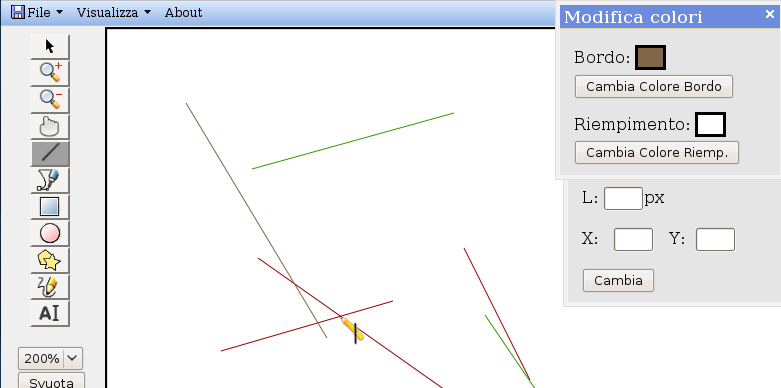
\includegraphics[scale=0.5]{images/linea.png}
\caption{Disegno di una retta}
\end{figure} 


\vspace{100pt}
Qui \`e stata selezionata la funzione \textit{Disegno di una retta}. Si deve premere il pulsante sinistro del mouse e spostare il cursore per disegnare la linea retta. La fine della retta \`e determinata dal rilascio del pulsante del mouse.

\newpage

\begin{figure}[!ht]
\centering
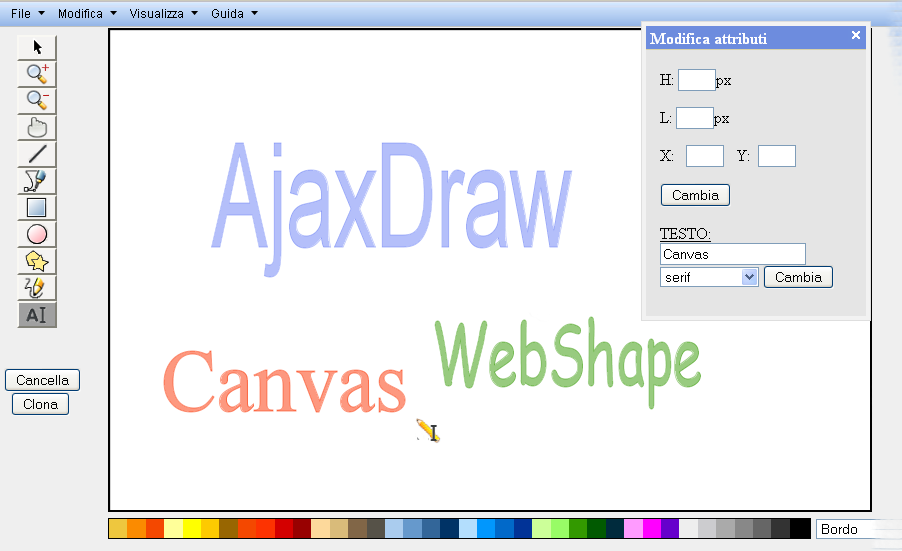
\includegraphics[scale=0.5]{images/label.png}
\caption{Etichetta di testo}
\end{figure} 


\vspace{100pt}
Qui \`e stata selezionata la funzione per la creazione di una\textit{casella di testo}. Si deve cliccare sull'area di disegno come per le altre figure, per stabilire posizione e dimensioni della casella,  ed utilizzare il dialog di propriet\`a per cambiare la stringa contenuta all'interno ed il tipo di carattere (solo per i browser che supportano tale funzionalit\` a).
\newpage

 
\begin{figure}[!ht]
\centering
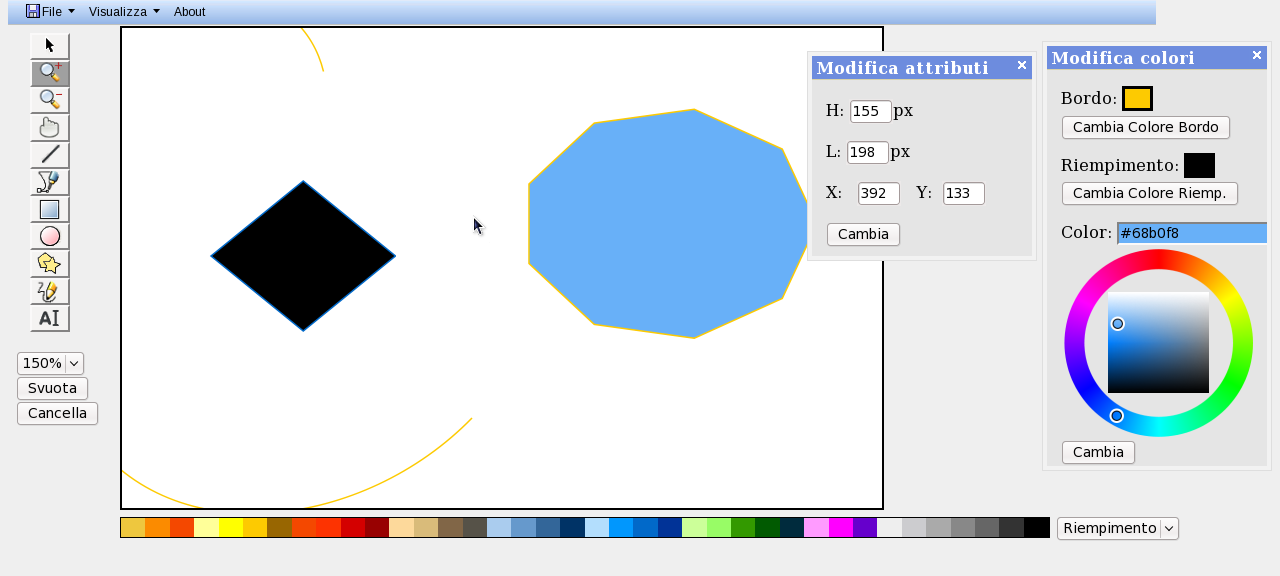
\includegraphics[scale=0.4]{images/zoom_piu.png}
\caption{Uso dello Zoom per ingrandimento al 150 per cento}
\end{figure} 

\begin{figure}[!ht]
\centering
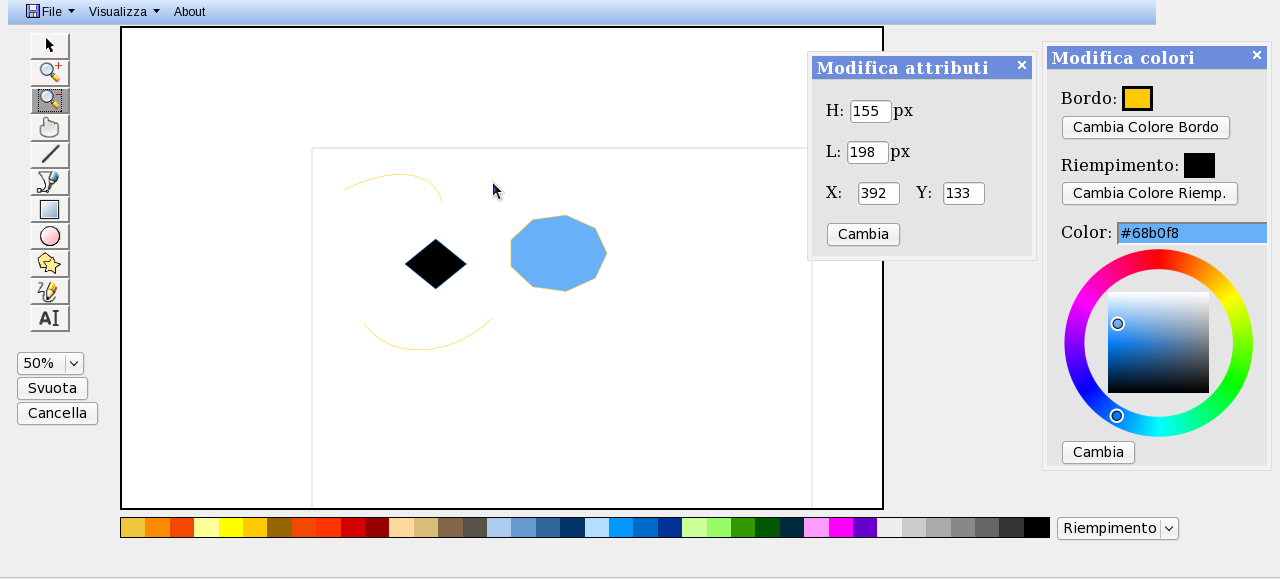
\includegraphics[scale=0.4]{images/zoom_meno.png}
\caption{Uso dello Zoom per diminuzione dell' ingrandimento al 50 per cento}
\end{figure} 

\vspace{100pt}
Qui \`e stata selezionata la funzione di \textit{Zoom}. \`E possibile aumentare o diminuire il livello di zoom mediante l'utilizzo dei pulsanti appositi.
 


\begin{figure}[!ht]
\centering
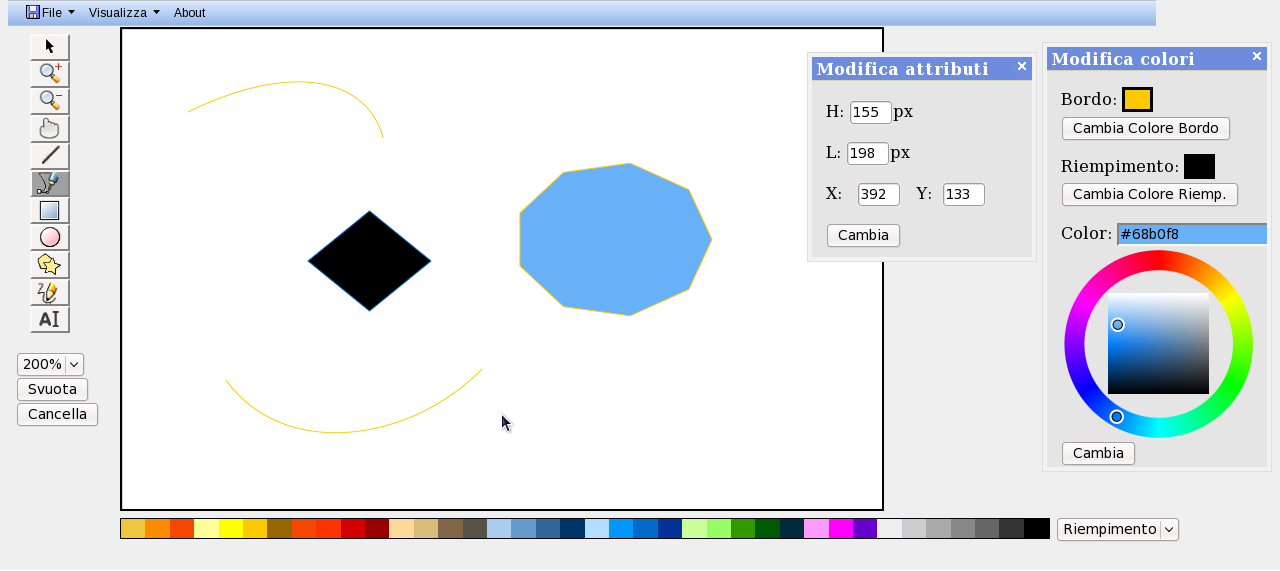
\includegraphics[scale=0.4]{images/bezier.png}
\caption{Disegno di una curva di bezier}
\end{figure} 

\vspace{100pt}

Qui \`e stata selezionata la funzione per il disegno di una \textit{Curva di Bezier} cubica. Per disegnare la curva, \` e necessario impostare i 4 punti necessari al suo calcolo. Il primo punto sar\`a l'inizio della curva, seguito dai due punti controllo per cui passeranno le tangenti ed infine l'ultimo imposter\` a il punto finale della curva. Si avr\` a comunque la possibilit\` a di controllare ad ogni passaggio la conformazione della figura in fase di creazione.

\newpage

%%%%%%%%%%%%%%%%%%%%%%%%%%%% FINE TOOLBAR %%%%%%%%%%%%%%%%%%%%%%%%%%%%%%%%

%%%%%%%%%%%%%%%%%%%%%%%%%%%% BOTTONI E DIALOG %%%%%%%%%%%%%%%%%%%%%%%%%%%%%%%%%
\subsubsezione{bottoni e finestre di dialogo}

\vspace{100pt}
Facendo click sul pulsante \textit{Svuota} in basso a sinistra, l'utente pu\`o cancellare tutto ci\`o che \`e stato di segnato sul piano di disegno fino a quel punto e ripartire da zero con un nuovo disegno. Si consiglia di salvare prima di cancellare per evitare di perdere il lavoro svolto finora.

\begin{figure}[!ht]
\centering
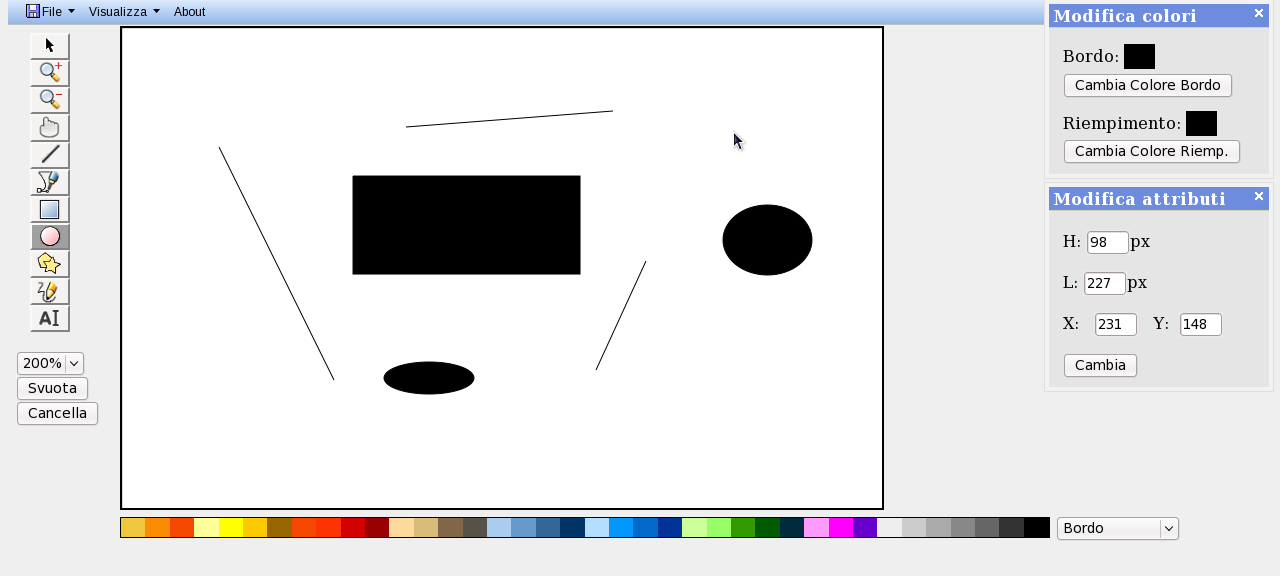
\includegraphics[scale=0.4]{images/cancella_elemento_prima.png}
\caption{Cancellazione di un elemento di disegno  - PRIMA}
\end{figure} 

\begin{figure}[!ht]
\centering
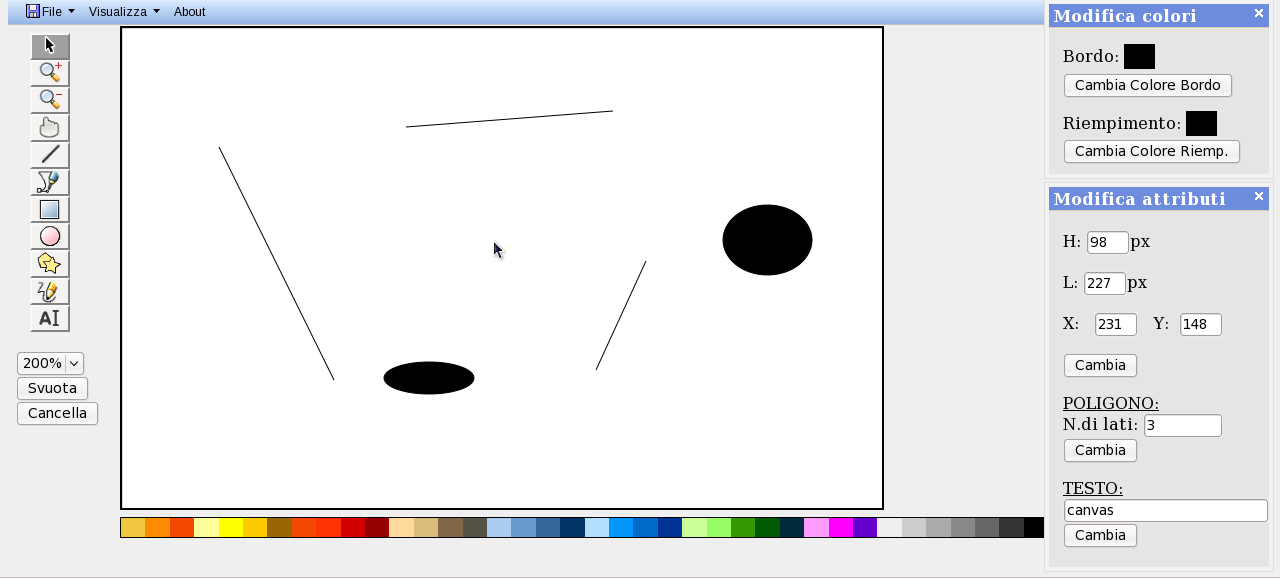
\includegraphics[scale=0.4]{images/cancella_elemento_dopo.png}
\caption{Cancellazione di un elemento di disegno  - DOPO}
\end{figure}

\vspace{100pt}
Il bottone \textit{Cancella} in basso a sinistra (sotto la toolbar di disegno) permette di cancellare una figura correntemente selezionata cliccando sul pulsante suddetto. La medesima funzione pu\`o essere svolta da tastiera premendo il tasto \textit{Canc}.

\begin{figure}[!ht]
\centering
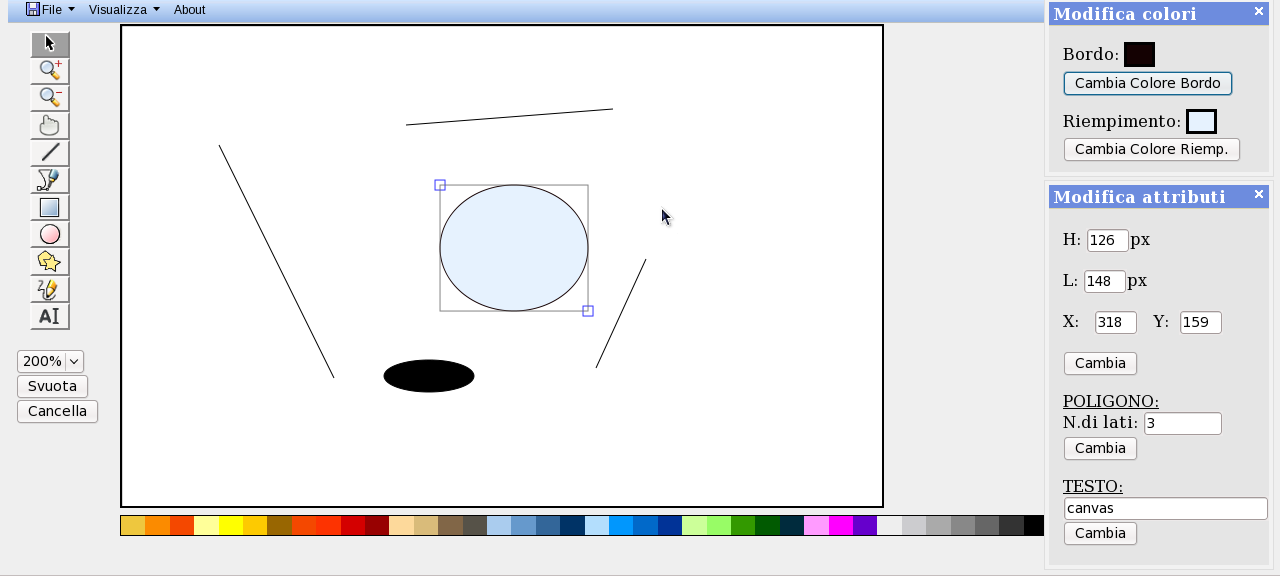
\includegraphics[scale=0.4]{images/colore_bordo_prima.png}
\caption{cambio colore del bordo  - PRIMA}
\end{figure} 

\begin{figure}[!ht]
\centering
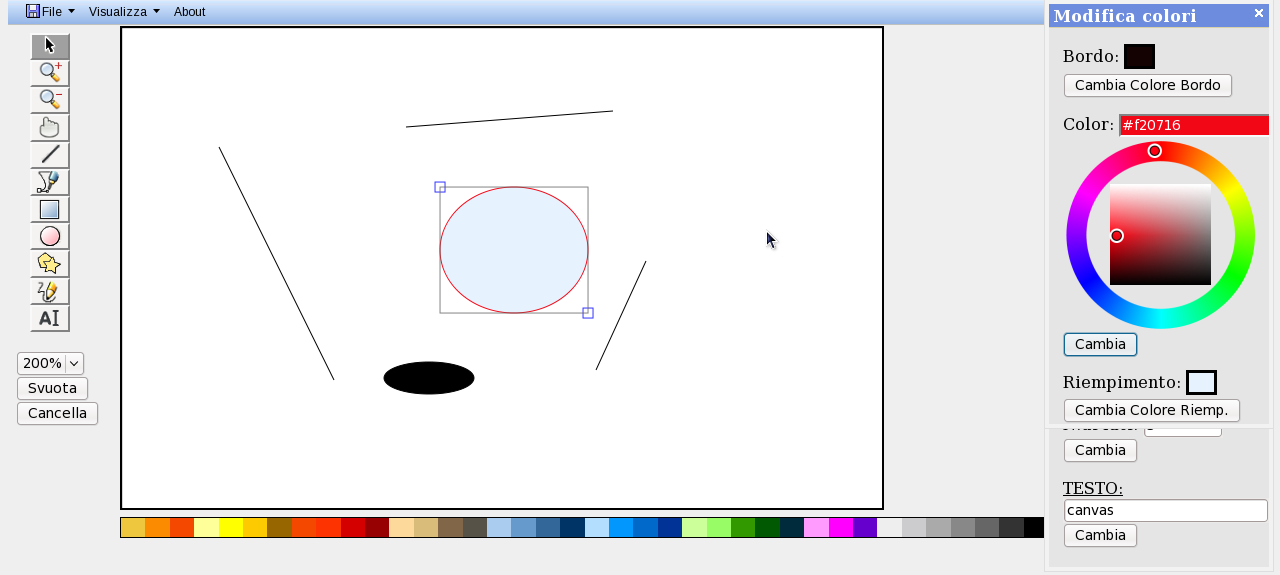
\includegraphics[scale=0.4]{images/colore_bordo_dopo.png}
\caption{cambio colore del bordo  - DOPO}
\end{figure} 


\vspace{100pt}
Qui \`e stata selezionata la funzione di cambiamento del colore del bordo della figura selezionata con l'ausilio del dialog \textit{Modifica Colori} posto in alto a destra. Per modificare il colore: 
\begin{elencopuntato}[\normindent]
\item[-] Cliccare sul pulsante \textit{Cambia Colore Bordo}.
\item[-] Appare sul dialog la ruota dei colori.
\item[-] Selezionare un colore a piacere sulla ruota e impostare il grado di opacit\`a dal rettangolo iscritto all'interno della ruota. 
\item[-]Quando il colore e l'opacit\`a sono stati scelti basta un click sul pulsante \textit{Cambia} per vedere il colore del contorno modificato con le tonalit\`a scelte. 
\end{elencopuntato}
Questa funzionalit\`a prevede la possibilit\`a per l'utente di cambiare il colore scegliendolo dalla \textit{Tavolozza} di colori posti sotto il piano di disegno: bisogna selezionare \textit{bordo} sulla combobox a destra della \textit{Palette} e cliccare sul colore scelto per cambiare il colore del bordo sul dialog. A questo punto basta un click sul pulsante \textit{Cambia Colore Bordo} e un click su \textit{Cambia}.

\begin{figure}[!ht]
\centering
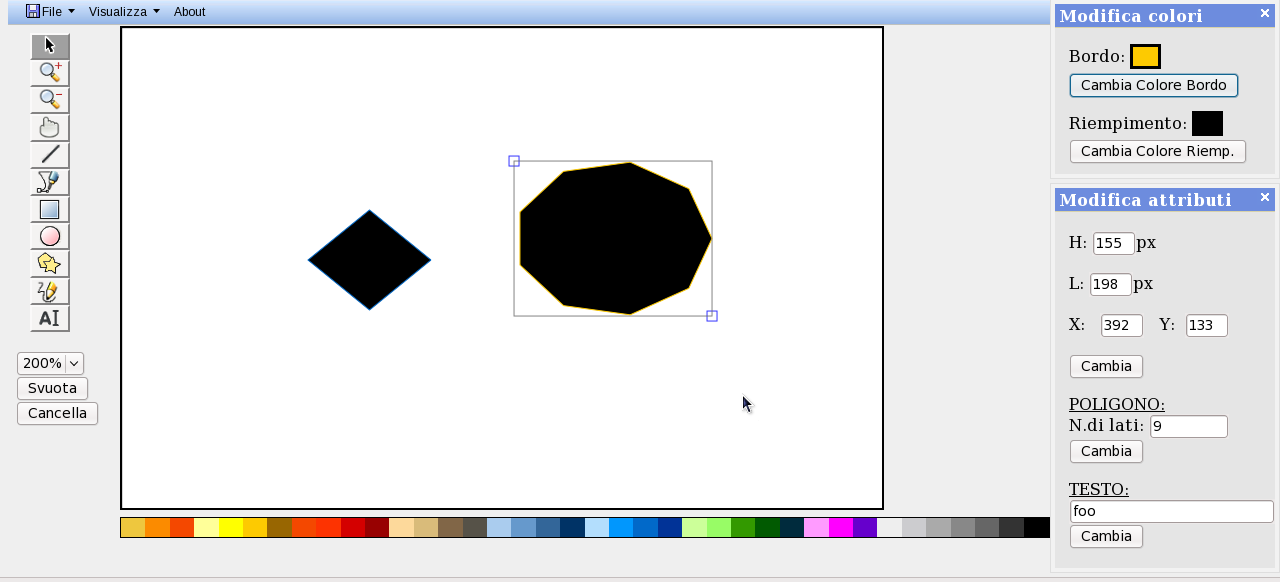
\includegraphics[scale=0.4]{images/colore_riempimento_prima.png}
\caption{cambio colore del riempimento  - PRIMA}
\end{figure} 

\begin{figure}[!ht]
\centering
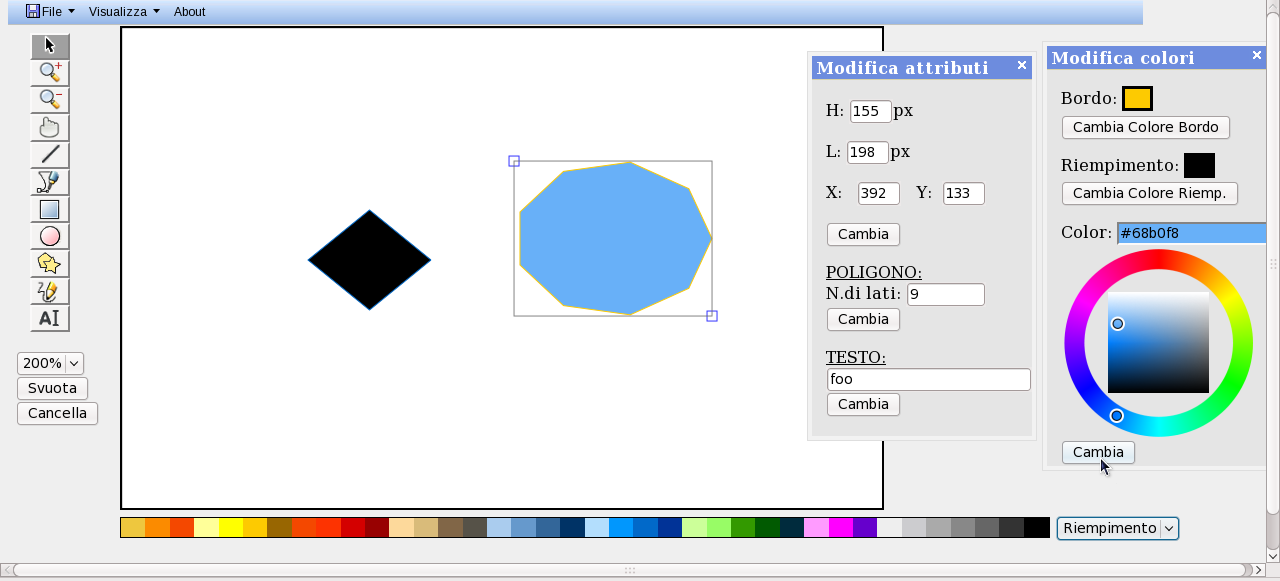
\includegraphics[scale=0.4]{images/colore_riempimento_dopo.png}
\caption{cambio colore del riempimento  - DOPO}
\end{figure} 


\vspace{100pt}
Qui \`e stata selezionata la funzione di cambiamento del colore di riempimento della figura selezionata con l'ausilio del dialog \textit{Modifica Colori} posto in alto a destra. Il funzionamento \`e completamente analogo a quanto descritto per modificare il colore del bordo. Non tutte le figure hanno un colore di riempimento.

\begin{figure}[!ht]
\centering
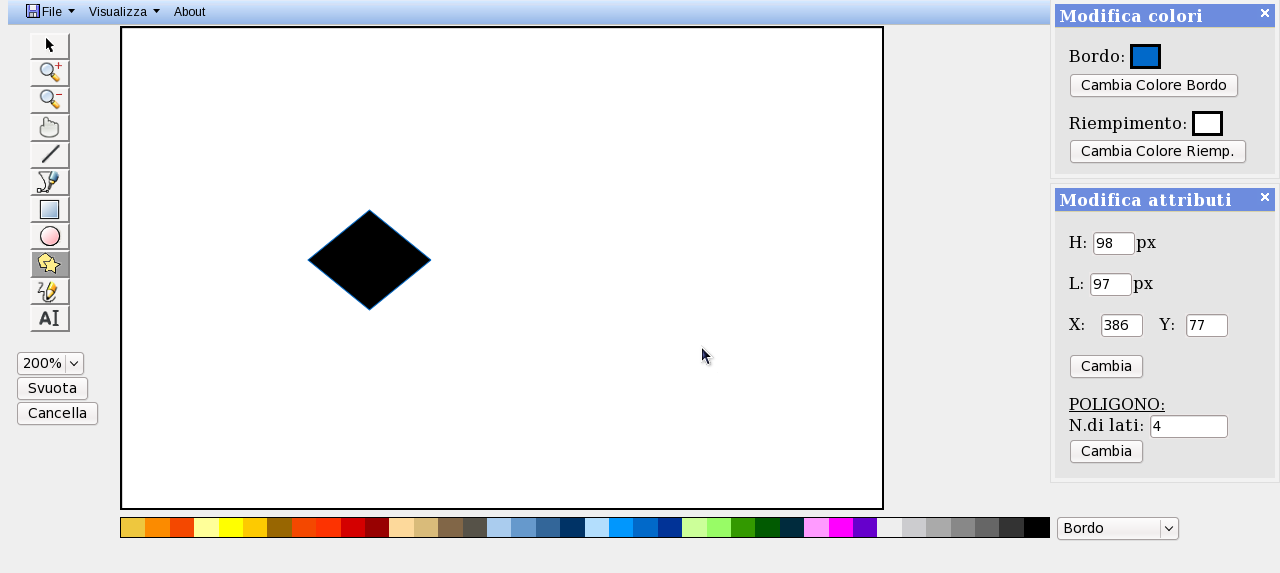
\includegraphics[scale=0.4]{images/numero_lati_prima.png}
\caption{cambio numero lati di un poligono  - PRIMA}
\end{figure} 

\begin{figure}[!ht]
\centering
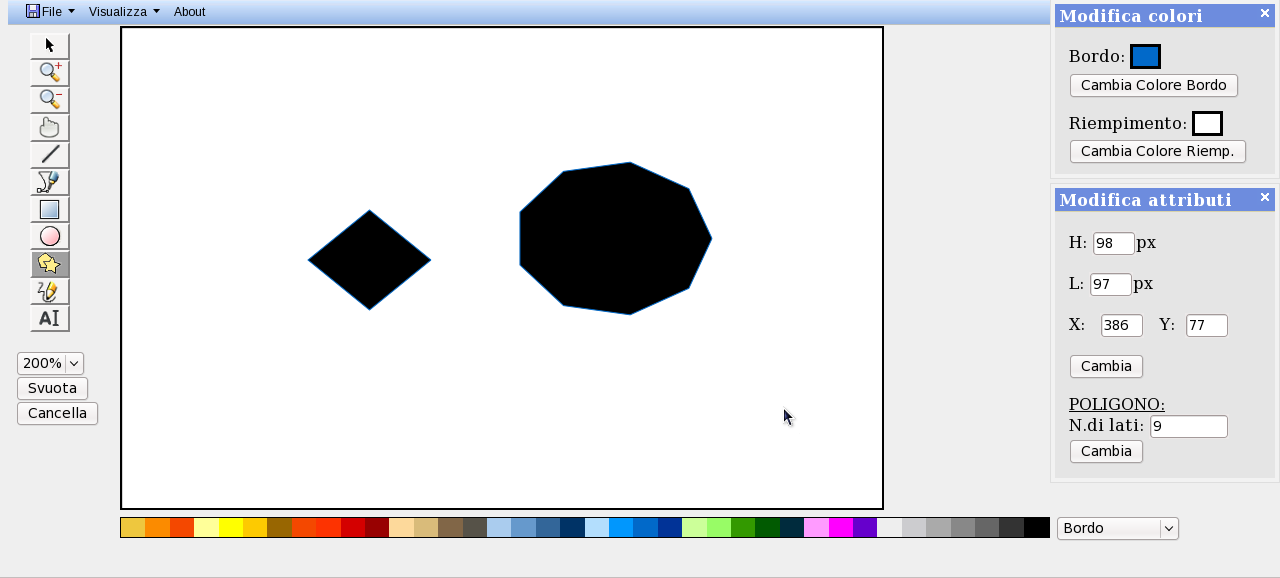
\includegraphics[scale=0.4]{images/numero_lati_dopo.png}
\caption{cambio numero lati di un poligono  - DOPO}
\end{figure} 

\vspace{100pt}
Qui \`e stata selezionata la funzione di cambiamento del numero di lati per il disegno di poligoni. Tale funzione viene gestita con l'ausilio del dialog \textit{Modifica Attributi} posto in alto a destra e precisamente nella parte riguardante il numero di lati. Modificando il valore e confermando cliccando sul pulsante a destra viene modificato il numero di lati del poligono correntemente selezionato e del prossimo poligono che verr\`a disegnato. \\

\begin{figure}[!ht]
\centering
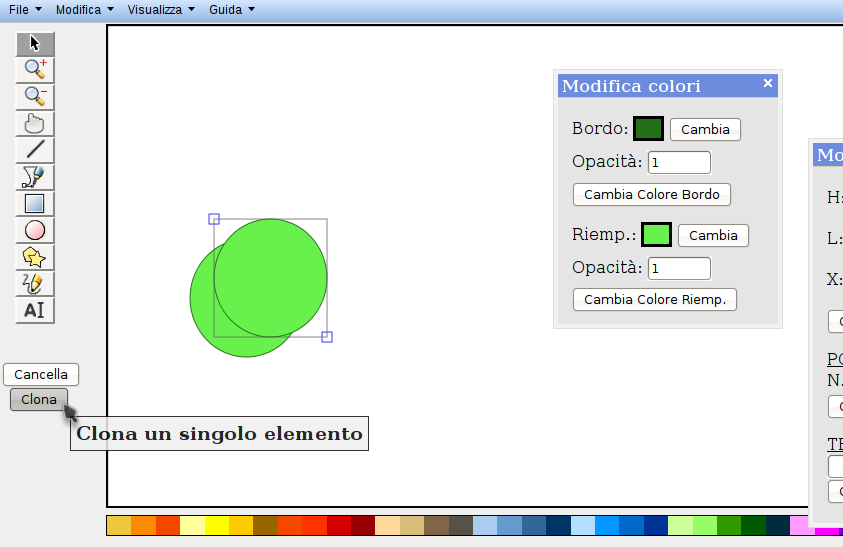
\includegraphics[scale=0.4]{images/clona.png}
\caption{cambio colore del bordo  - PRIMA}
\end{figure} 

\begin{figure}[!ht]
\centering
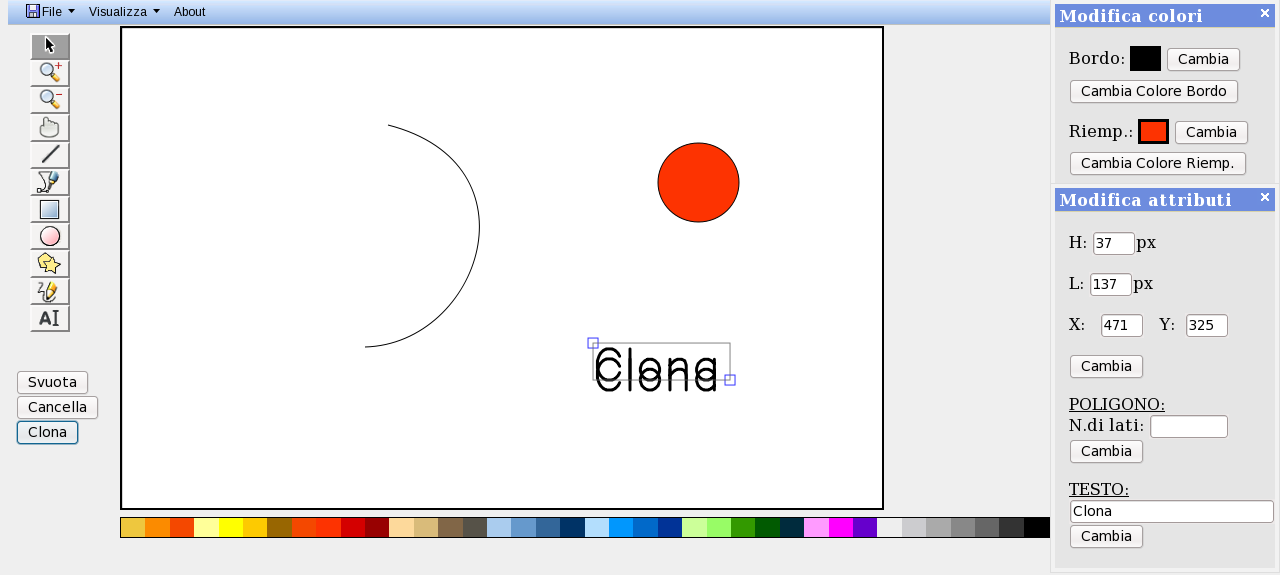
\includegraphics[scale=0.4]{images/clona_dopo.png}
\caption{cambio colore del bordo  - DOPO}
\end{figure} 

\vspace{100pt}
Qui \`e stata selezionata la funzione di clonazione di un oggetto presente sul piano di disegno e precedentemente selezionato. Tale funzione permette di fare una copia di tutti gli oggetti disegnabili mediante un semplice click sul pulsante apposito \textit{Clona} posto in basso a sinistra. \\

\sezione{Appendice}

\subsezione{Messaggi di errore e loro significato}
descrizione degli errori, dividendoli tra server e \underline{client}\\
Errore di \underline{parsing} durante il caricamento di un file SVG.\\
Errore di comunicazione col server. \\
Errore interno del server (e.g. non c'e' piu' spazio su disco).\\

\end{document}
